%%%%%%%%%%%%%%%%%%%%%%%%%%%%%%%%%%%%%%%%%
% Beamer Presentation
% LaTeX Template
% Version 1.0 (10/11/12)
%
% This template has been downloaded from:
% http://www.LaTeXTemplates.com
%
% License:
% CC BY-NC-SA 3.0 (http://creativecommons.org/licenses/by-nc-sa/3.0/)
%
%%%%%%%%%%%%%%%%%%%%%%%%%%%%%%%%%%%%%%%%%

%----------------------------------------------------------------------------------------
%	PACKAGES AND THEMES
%----------------------------------------------------------------------------------------

\documentclass{beamer}

\mode<presentation> {

% The Beamer class comes with a number of default slide themes
% which change the colors and layouts of slides. Below this is a list
% of all the themes, uncomment each in turn to see what they look like.

%\usetheme{default}
%\usetheme{AnnArbor}
%\usetheme{Antibes}
%\usetheme{Bergen}
%\usetheme{Berkeley}
%\usetheme{Berlin}
%\usetheme{Boadilla}
%\usetheme{CambridgeUS}
%\usetheme{Copenhagen}
%\usetheme{Darmstadt}
%\usetheme{Dresden}
%\usetheme{Frankfurt}
%\usetheme{Goettingen}
%\usetheme{Hannover}
%\usetheme{Ilmenau}
%\usetheme{JuanLesPins}
%\usetheme{Luebeck}
\usetheme{Madrid}
%\usetheme{Malmoe}
%\usetheme{Marburg}
%\usetheme{Montpellier}
%\usetheme{PaloAlto}
%\usetheme{Pittsburgh}
%\usetheme{Rochester}
%\usetheme{Singapore}
%\usetheme{Szeged}
%\usetheme{Warsaw}

% As well as themes, the Beamer class has a number of color themes
% for any slide theme. Uncomment each of these in turn to see how it
% changes the colors of your current slide theme.

%\usecolortheme{albatross}
%\usecolortheme{beaver}
%\usecolortheme{beetle}
%\usecolortheme{crane}
%\usecolortheme{dolphin}
%\usecolortheme{dove}
%\usecolortheme{fly}
%\usecolortheme{lily}
%\usecolortheme{orchid}
%\usecolortheme{rose}
%\usecolortheme{seagull}
%\usecolortheme{seahorse}
%\usecolortheme{whale}
%\usecolortheme{wolverine}

%\setbeamertemplate{footline} % To remove the footer line in all slides uncomment this line
%\setbeamertemplate{footline}[page number] % To replace the footer line in all slides with a simple slide count uncomment this line

%\setbeamertemplate{navigation symbols}{} % To remove the navigation symbols from the bottom of all slides uncomment this line
}

\usepackage{graphicx} % Allows including images
\usepackage{booktabs} % Allows the use of \toprule, \midrule and \bottomrule in tables
\usepackage{subcaption}

\def\indep{\perp \!\!\! \perp}

%----------------------------------------------------------------------------------------
%	TITLE PAGE
%----------------------------------------------------------------------------------------

\title[Macro DAGs]{DAGs with Applications to Macroeconomic Timeseries} % The short title appears at the bottom of every slide, the full title is only on the title page

\author{Emmet Hall-Hoffarth} % Your name
\institute[Oxford] % Your institution as it will appear on the bottom of every slide, may be shorthand to save space
{
University of Oxford \\ % Your institution for the title page
\medskip
\textit{emmet.hall-hoffarth@economics.ox.ac.uk} % Your email address
}
\date{\today} % Date, can be changed to a custom date

\begin{document}

\begin{frame}
    \titlepage % Print the title page as the first slide
\end{frame}

\begin{frame}
    \frametitle{Overview} % Table of contents slide, comment this block out to remove it
    \tableofcontents % Throughout your presentation, if you choose to use \section{} and \subsection{} commands, these will automatically be printed on this slide as an overview of your presentation
\end{frame}

\section{Background}

\subsection{DAGs}
\subsubsection{Representation}
\begin{frame}
    \frametitle{DAGs}
    \begin{tabular}{ p{5.5cm} p{5.5cm} }
        \begin{figure}
            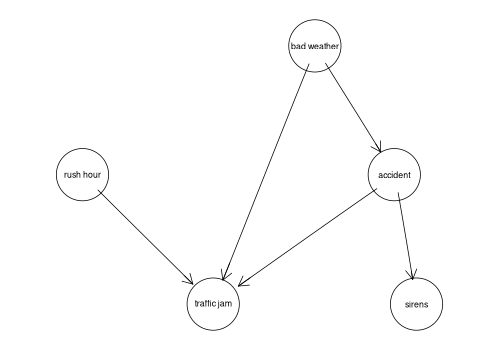
\includegraphics[width=4.5cm]{images/trafficjam.png}
            \caption{An example of a simple DAG}
            \label{dag1}
        \end{figure}
        &
        \begin{itemize}
            \item Root nodes of the graph are $i.i.d.$ shocks.
            \item Parent nodes are exogenous relative to their children.
            \item Each arc specifies a (generic) conditional probability relationship.
            \item I will assume that the data follows a joint normal distribution $s.t.$ each conditional probability relationship is a linear function with a normally distributed error.
        \end{itemize}
    \end{tabular}
\end{frame}

\subsubsection{Structure learning}
\begin{frame}
    \frametitle{Structure Learning}
    \begin{figure}
        \centering
        \begin{subfigure}{0.3\textwidth}
          \centering
          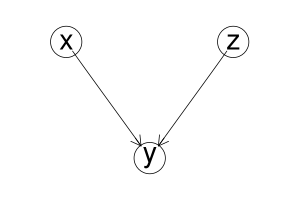
\includegraphics[width=\linewidth]{images/collider.png} 
          \small
          \begin{equation*}
            x = \epsilon_{x}
          \end{equation*}
          \begin{equation*}
            y = \beta_{yx} x + \beta_{yz} z + \epsilon_{y}
          \end{equation*}
          \begin{equation*}
            z = \epsilon_{z}
          \end{equation*}
          \caption{Collider}
          \label{collider}
        \end{subfigure}
        %
        \begin{subfigure}{0.3\textwidth}
          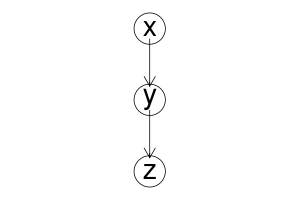
\includegraphics[width=\linewidth]{images/chain.png}
          \small
          \begin{equation*}
            x = \epsilon_{x}
          \end{equation*}
          \begin{equation*}
            y = \beta_{yx} x + \epsilon_{y}
          \end{equation*}
          \begin{equation*}
            z = \beta_{zy} y + \epsilon_{z}
          \end{equation*}
          \caption{Chain}
          \label{chain}
        \end{subfigure}
        %
        \begin{subfigure}{0.3\textwidth}
          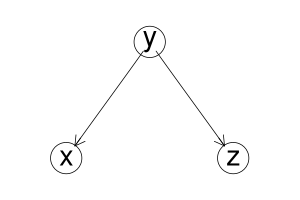
\includegraphics[width=\linewidth]{images/fork.png}
          \small
          \begin{equation*}
            x = \beta_{xy} y + \epsilon_{x}
          \end{equation*}
          \begin{equation*}
            y = \epsilon_{y}
          \end{equation*}
          \begin{equation*}
            z = \beta_{zy} y + \epsilon_{z}
          \end{equation*}
          \caption{Fork}
          \label{fork}
        \end{subfigure}
        \caption{The three possible v-structures of a 3 node DAG. Error terms $\epsilon$ are all i.i.d. Gaussian shocks.}
        \label{dag2}
      \end{figure}
\end{frame}

\begin{frame}
    \frametitle{Structure Learning}
    \begin{itemize}
        \item These three V-structures are partially identifiable because they have different testable implications about conditional (in)dependence.
        \begin{itemize}
            \item Collider $\implies x \indep z$ but $x \not\!\indep z | y$
            \item Chain $\implies x \not\!\indep z$ but $x \indep z | y$
            \item Fork $\implies x \not\!\indep z$ but $x \indep z | y$
        \end{itemize}
        \item In the context of a linear Gaussian model these conditional (in)dependence relationships can be tested with a t-test.
        \item Many algorithms have been developed which use this basic idea to identify (to the greatest extent possible) the underlying DAG given observed data. This are \textit{Constraint-Based Algorithms}.
        \item There are also \textit{Score-Based Algorithms} that maximise a score (eg. likelihood) over the set of possible DAGs using gradient decent, and \textit{Hybrid Algorithms} that combine both approaches.
    \end{itemize}
\end{frame}

\subsection{DSGE}
\begin{frame}
    \frametitle{DSGE}
    \begin{tabular}{ p{5cm} p{5cm} }
        \begin{figure}
            \centering
            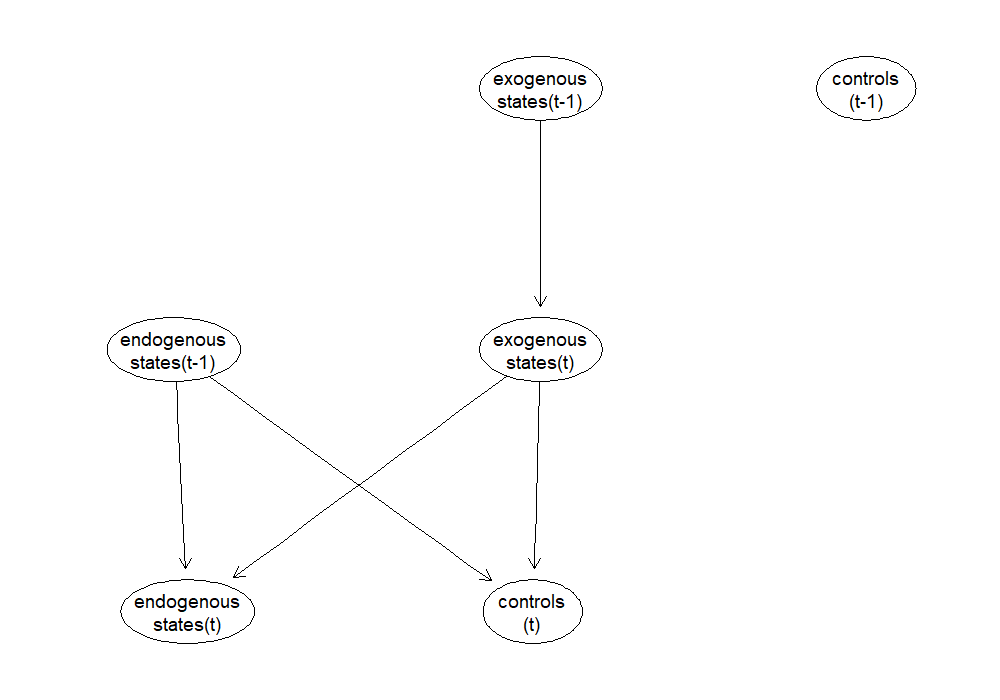
\includegraphics[width=5cm]{images/dsge_dag.png}
            \caption{The general solution to a DSGE model as a DAG}
            \label{dag3}
          \end{figure}
        &
        \begin{itemize}
            \item Exogenous states: Current value determines current state of model and depends only on its own past. (eg. technology)
            \item Endogenous states: Current value depends on states, but past values determine current state of model. (eg. capital)
            \item Controls: Current value depends on states, past values are irrelevant. (eg. consumption)
        \end{itemize}
    \end{tabular}
\end{frame}

\begin{frame}
    \frametitle{DSGE}
    \begin{itemize}
        \item The DAG on the previous slide defines the \textit{ground-truth} that we seek to identify from data generated by a DSGE simulation.
        \item Structure learning provide asymptotic theoretical guarantees that they can identify the ground truth given some observational data.
        \item This model is essentially a regularised ADL regression. Therefore, structure learning provides an agnostic way to regularise and choose contemporaneous regressors for the ADL model. 
        \item So everything is in order then?
    \end{itemize}
\end{frame}

\section{Application}
\subsection{RBC}
\begin{frame}
    \frametitle{Application}
    \begin{tabular}{ p{5cm} p{5cm} }
        \begin{figure}
            \centering
            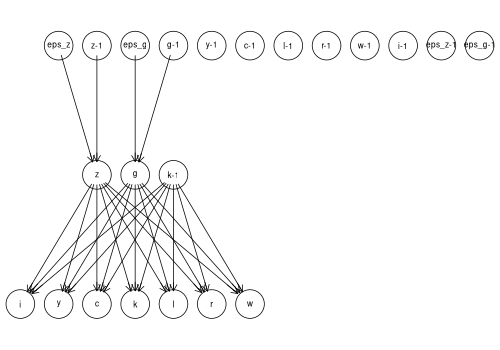
\includegraphics[width=5cm]{images/rbc_true_dag.png}
            \caption{Ground truth solution to RBC model}
            \label{dag4}
          \end{figure}
        &
        \begin{figure}
            \centering
            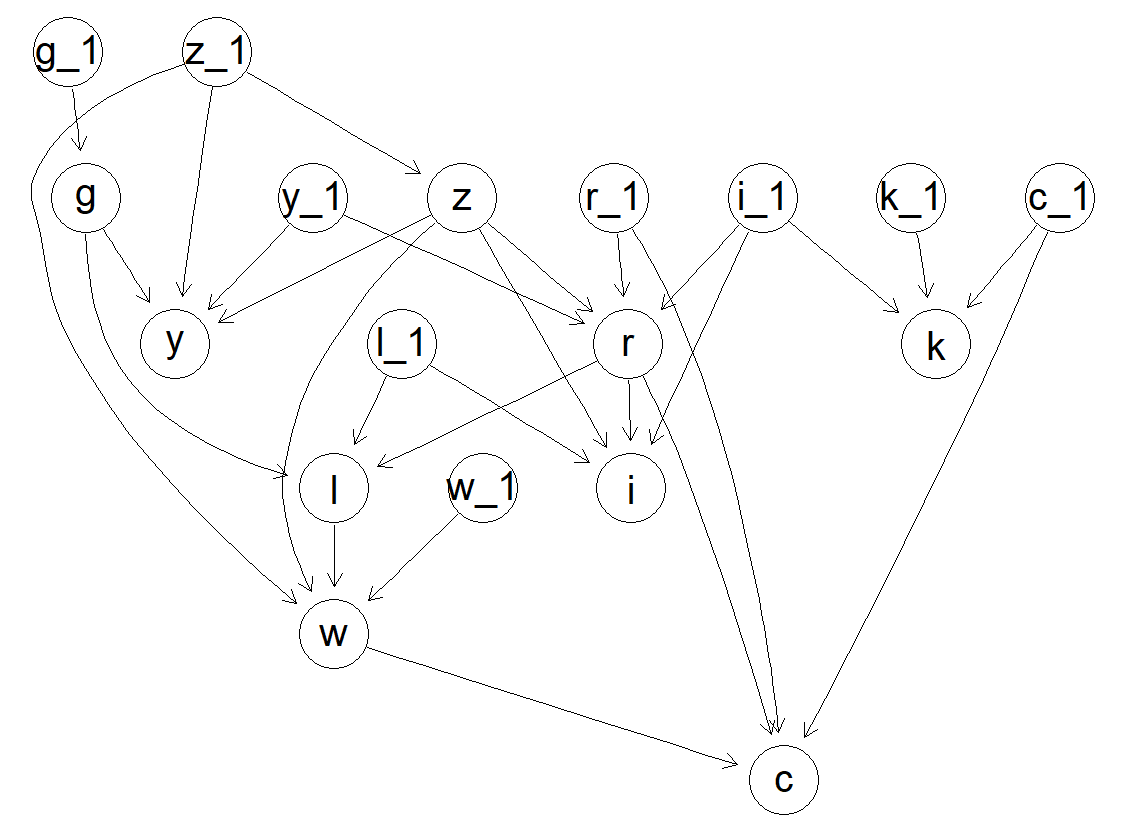
\includegraphics[width=5cm]{images/rbc_hybrid_structure.png}
            \caption{Estimated DAG for RBC data (hybrid algorithm, 100k observations)}
            \label{dag5}
          \end{figure}
    \end{tabular}
\end{frame}

\begin{frame}
    \frametitle{Application}
    \begin{itemize}
        \item Not quite....
        \item There seeems to be a number of problems with these algorithms, especially using simulated data:
        \begin{itemize}
            \item Faithfulness: We require that every dependency in the underlying DGP correspond to an observed statistical dependence. This is violated if some effects cancel out resulting in no observed correlation (eg mon. auth. chooses interest rate to cancel effect of inflationary shock on output)
            \item Collinearity: Calculating conditional correlation requires calculating regression residuals. In simulation, these are very close to zero conditional on the correct states, so the computation is unstable.
            \item Asymptotics: The problem space grows super-exponentially with the number of variables $\implies$ even a sample size of 100k may not be big enough for asymptotic arguments.
        \end{itemize}
    \end{itemize}
\end{frame}

\begin{frame}
    \frametitle{Application}
    \begin{tabular}{ p{5cm} p{5cm} }
        \begin{figure}
            \centering
            \begin{subfigure}{5cm}
              \centering
              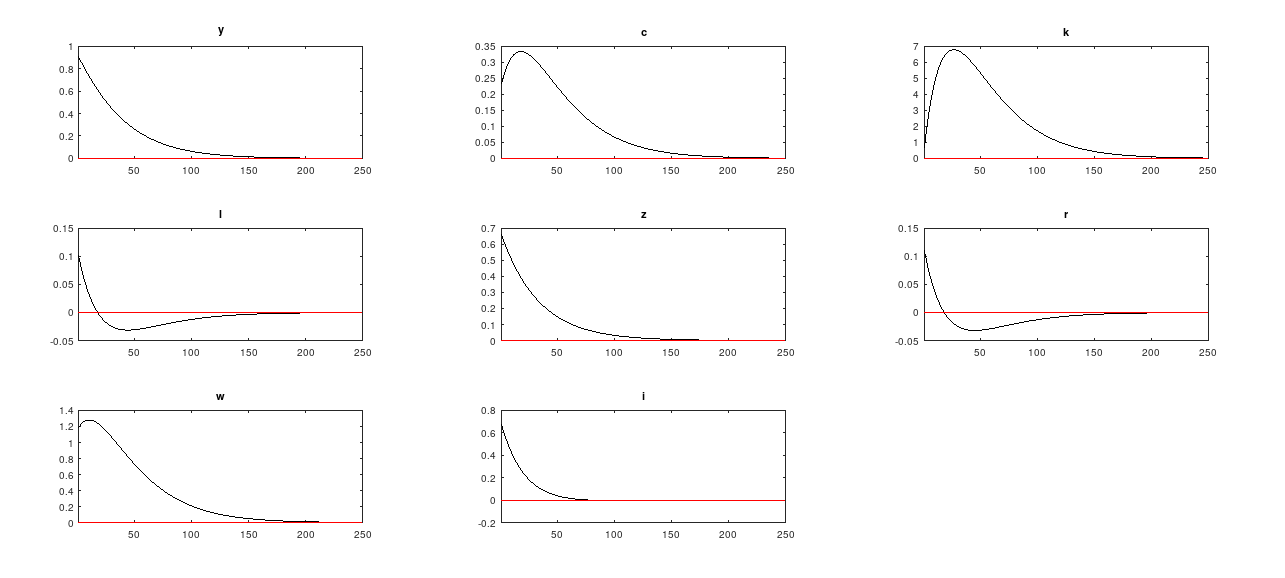
\includegraphics[width=\linewidth, height=1.25cm]{images/rbc_sim_irf.png} 
              \caption{Original Simulation}
              \label{simirf}
            \end{subfigure}
            %
            \begin{subfigure}{5cm}
              \centering  
              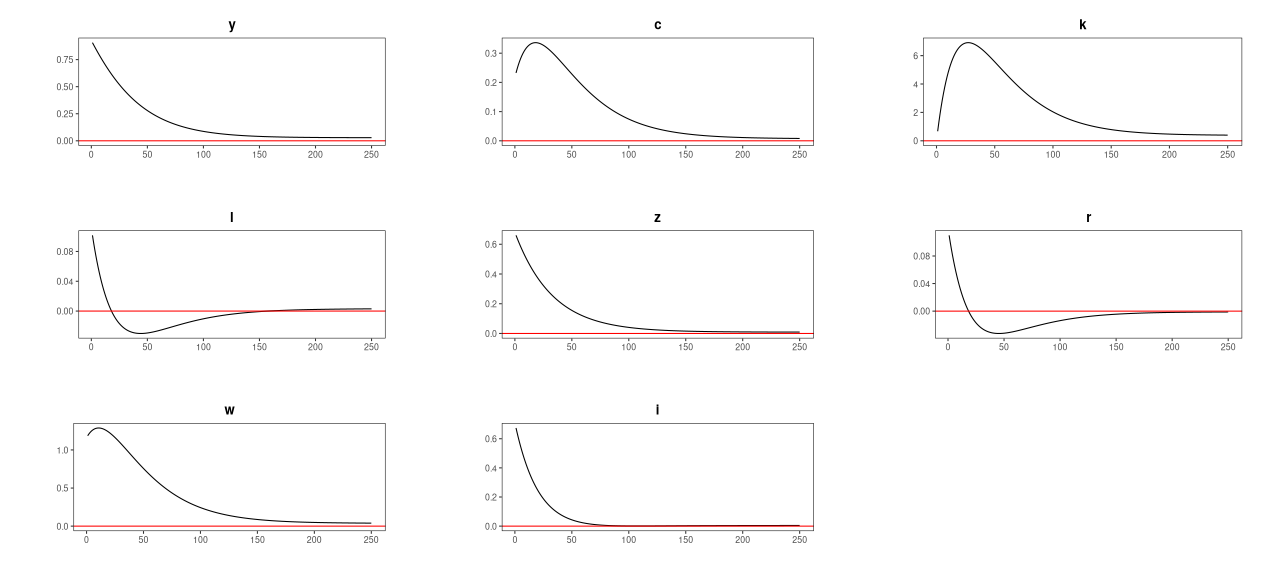
\includegraphics[width=\linewidth, height=1.25cm]{images/rbc_true_dag_irfs.png}
              \caption{Ground Truth DAG}
              \label{gtirf}
            \end{subfigure}
            %
            \begin{subfigure}{5cm}
              \centering  
              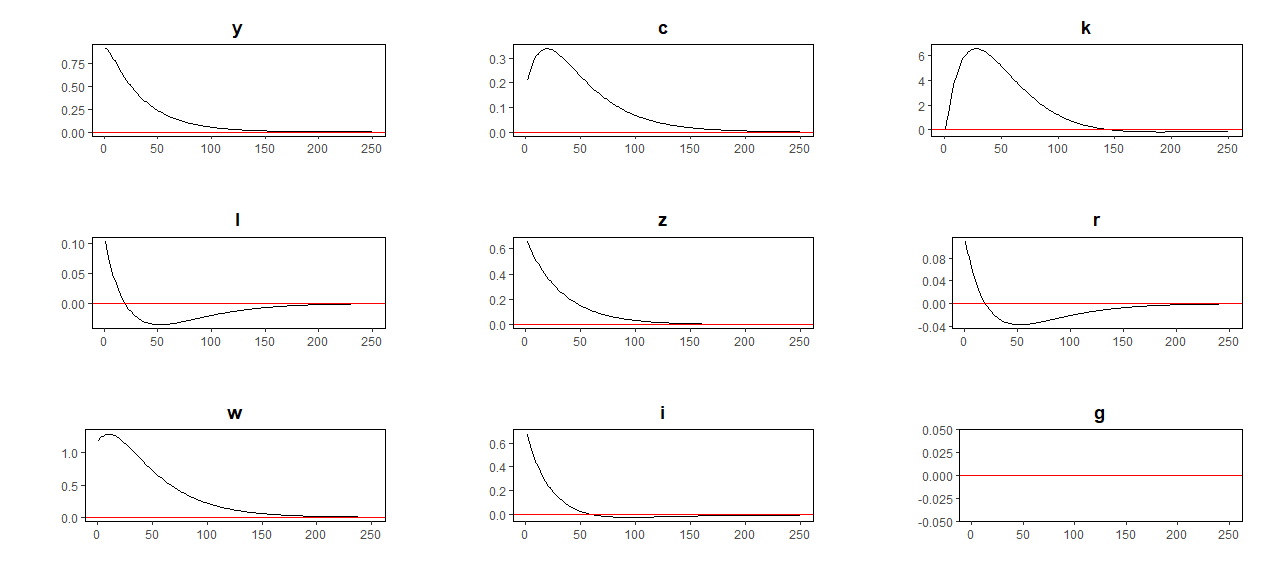
\includegraphics[width=\linewidth, height=1.25cm]{images/rbc_hybrid_irfs.png}
              \caption{Fitted DAG (Hybrid Algorithm)}
              \label{hirf}
            \end{subfigure}
            \caption{IRFs to a one standard deviation technology shock.}
            \label{dag10}
        \end{figure}
        &
        \begin{itemize}
            \item Even if structure learning does not return the ground-truth it does (sometimes) return a model that is causally equivalent in the sense that correctly identifies the states and replicates the true IRFs.
            \item Furthermore, when using real data concerns about faithfulness, collinearity, and even asymptotics (if we consider a small number of variables) are less pronounced...
        \end{itemize}
    \end{tabular}
\end{frame}

\subsection{Real data}
\begin{frame}
    \frametitle{Application}
    \begin{tabular}{ p{5cm} p{5cm} }
        \begin{figure}
            \centering
            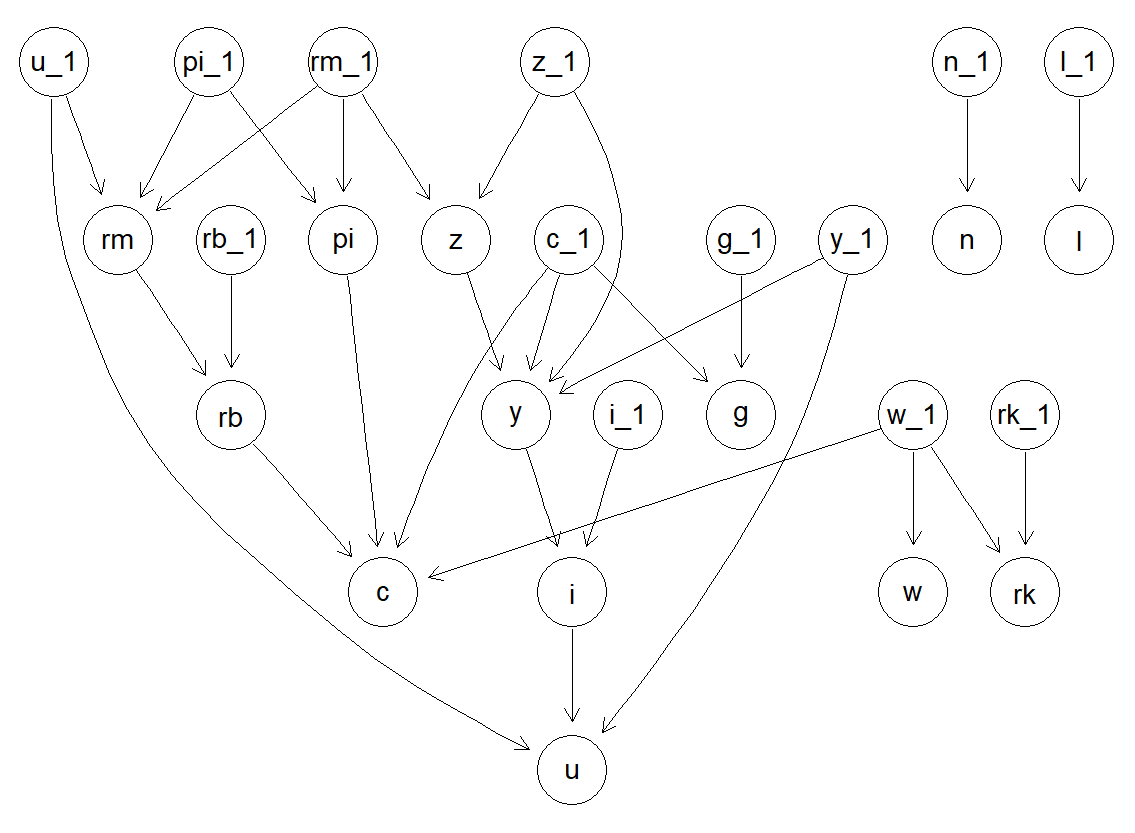
\includegraphics[width=5cm]{images/real_hybrid_structure.png}
            \caption{Estimated DAG for US economy 1980-2005 (hybrid algorithm)}
            \label{dag4}
          \end{figure}
        &
        \begin{figure}
            \centering
            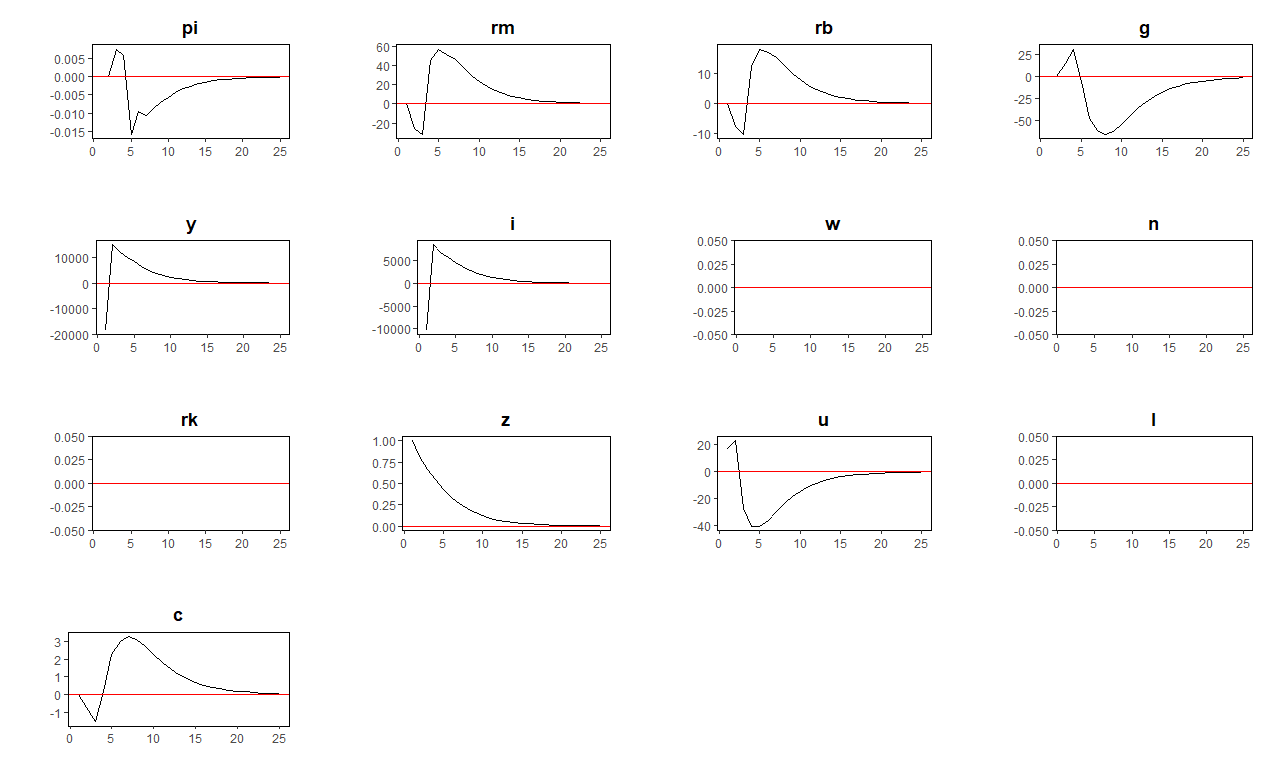
\includegraphics[width=5cm,height=4cm]{images/real_z_irf.png}
            \caption{IRFs to TFP shock for estimated DAG}
            \label{dag5}
          \end{figure}
    \end{tabular}
\end{frame}

\begin{frame}
    \frametitle{Application}
    \begin{itemize}
        \item Since there is no ground-truth availible we can consider this DAG against commonly accepted stylised facts.
        \item The parents of $rm$, other than its own lag are $u_{t-1}$ and $\pi_{t-1}$ suggesting Taylor Rule like behaviour. There is a causal pathway from past monetary policy into current unemployment implying that monetary policy is a viable stabilising tool. 
        \item $n$ and $l$ are separate from the rest of the graph suggesting the exogeneity of these variables, which is entirely reasonable. 
        \item $z_t$ feed directly into $y_t$, $w_{t-1}$ into $c_t$, and $i_t$ into $u_t$, all of which seem like plausible causal linkages.
        \item The IRFs seem to reflect many stylised facts about the macroeconomy in terms of direction of effect, even if the implied responses leave something to be desired, especially with regards to their jagged shape. 
    \end{itemize}
\end{frame}

\section{Papers to Write}

\subsection{DSGE-specific strucuture learning}
\begin{frame}
    \frametitle{DSGE-Specific Structure Learning}
    \begin{itemize}
        \item Another problem with existing structure learning algorithms is that they are \textit{too agnostic} relative to what we are willing to assume in this context. 
        \item If the DAG is a solution to a DSGE model it must take on a specific form, as illustrated in Figure \ref{dag3}.
        \item By explicitly assuming the resulting DAG takes on this form we can drastically reduce the size of the search space and likely greatly improve the resulting estimated DAG.
        \item I have already implemented this, and the only significant roadblock seems to be the collinearity issue as discussed earlier.
    \end{itemize}
\end{frame}

\subsection{Real data}
\begin{frame}
    \frametitle{Focus on Real Data}
    \begin{itemize}
        \item The original idea of this research was to use simulated data to give credence to the application to real data.
        \item As it turns out there are many problems with simulated data the appear to not be an issue for real data.
        \item This suggestion, therefore, is to ignore the simulations and instead provide a number of real data applications in the paper and evaluate those models against well-understood intuitions.
    \end{itemize}
\end{frame}

\subsection{Choose your own states}
\begin{frame}
    \frametitle{"Choose your own states adventure"}
    \begin{itemize}
        \item If a DSGE-like solution is assumed, a researcher needs only to choose what they assume to be the exogenous and endogenous states in order to estimate a model.
        \item I propose a methodology whereby researchers first test different combinations of states to see whether they produce expected IRFs, and only then go to develop a structural model that contains those states.
        \item This approach is data-driven and mostly agnostic, as apposed to the \textit{ad hoc} approach that is commonly employed.
    \end{itemize}
\end{frame}

\section{Conclusion}
\begin{frame}
    \frametitle{Conclusion}
    \begin{itemize}
        \item DAGs can allow for agnostic, data-driven discovery of causal models, and there are likely many applications in economics where this will prove useful.
        \item My research aims to demonstrate one such applicaion by utilizing macroeconomic timeseries data.
        \item While initial results have been mixed, DAGs do so some promise, especially as a regularisation technique.
        \item The exact direction of the paper(s) that I will write on these topics has yet to be determined.
    \end{itemize}
\end{frame}

\end{document} 